
The Dynamic Alignment List (DAL) is an abstract datatype designed to organize the relations (relational couplers) between videos as well to provide the features required to store and process the relations. Each relation stored into a DAL instance corresponds to a relational coupler related with a pair of video streams and the $\Delta{time}$ between them.


The start model for the storage structure inside the DAL was a relational matrix MxM which can represent all possible relations between M videos, each position representing the $\Delta{time}$ between the initial point of a pair of videos. This matrix was reduced to a upper triangular matrix because $\forall{i,j} < M , \Delta_{i,j}$ = $- \Delta_{j,i}$ and the main diagonal was eliminated because $\Delta_{i,j}$ is always equal to zero. The $\Delta{time}$ for each couple of videos is calculated for $\Delta{i,j} = start(j) - start(i)$ where $start(X)$ returns the offset of video X from the start of the event's timeline.

These values are used to synchronize the M videos. If $\Delta{i,j} > 0$ the video $i$ starts before the video $j$, if $\Delta{i,j} < 0$ the video $i$ starts after the video $j$, and when $\Delta{i,j} = 0$ both videos start at the same time. The values are represented in milliseconds, so $\Delta{i,j} = 30$ means the video $j$ should starts 30 ms after the video $i$ starts in order to achieve their synchronization. Additionally, in cases which is impossible to determine a relation between a pair of videos, the value registered is $I$ that means impossible.

Into a collaborative scenario where users can contribute providing a $\Delta{i,j}$ for a pair of videos $(i,j)$, it is important to store all contributions, because the $\Delta{time}$ value should be calculated considering the contributions collected for that pair. In that approach the formula $\Delta{i,j} = start(j) - start(i)$  is used to calculate the $\Delta{time}$ for each contribution, and the value stored in DAL is determined processing all contributions for each pair. Moreover, the number of contributions for each pair can grow while the contribution process is active, and current $\Delta{time}$ of a pair can change while contributions are incoming.

In order to represent this model it was needed to define a structure more sophisticated then a matrix. This structure preserves the relational characteristics of a upper triangular matrix without the main diagonal, with an additional dimension related to the contributions for each relation between video pairs. However, it is implemented as a hash table, using linked lists hierarchically organized in three levels. 

\begin{itemize}

\item Level 1 - The first level is a list of video structures. Each structure has a unique identification label for a correspondent video. 

\item Level 2 - Each video structure points to a second level linked list composed by all possible relations that include its video, considering the relations in a upper triangular matrix without the main diagonal.  Thus, each node in a second level linked list corresponds to a relation between it's video represented in its root and another video.

\item Level 3 - Each relation in a level 2 list points to a third level list, in which each node represent a contribution for that relation.

\end{itemize}

Figure~\ref{dal} exemplify a data structure into a DAL with 5 videos. The videos, labeled as $A, B, C, D$  and $E$, are in the fist level linked list. Each video points to a second level list, it is possible to observe in Figure~\ref{dal}  that each second level linked list have only the relations that would exist in a single line of a upper triangular matrix without the main diagonal. Moreover, in Figure~\ref{dal} each relation, that is an element of second level list, points to a cloud that represents a third level list with all contributions for that relation.

\begin{figure}
	\centering
	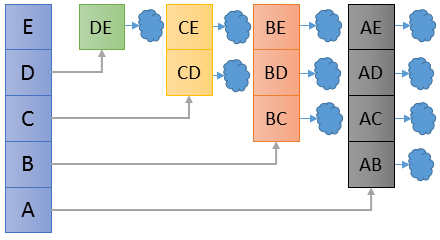
\includegraphics[scale=0.8]{figures/dal}
	\caption{DAL with 5 Videos (A,B,C,D,E)}
	\label{dal}
\end{figure}

A completed DAL can provide all information needed to achieve synchronization for videos registered on it, although it is more than a data structure. DAL is an abstract datatype that provides the data structure plus a set of features that allows access, manage and process the information inside it, such as the function \textit{Infer Synchronization}. 

\textit{Infer Synchronization} can obtain additional relations by executing an inference algorithm over the current relations. This algorithm checks if is possible to find an indirect path between two videos by transitivity. For example, considering the videos $A, B$ and $C$, if the relations $AB$ and $BC$ are known, by transitivity is possible to infer the relation $AC$. This feature can reduce the number of contributions required to complete a DAL. 



